% Inverse loop fixture: a.tex with a positioned text box, a smaller picture and new notes.
\documentclass{beamer}
\setbeamertemplate{navigation symbols}{}
\usepackage[absolute,overlay]{textpos}
\graphicspath{{img/}}
\title{Inverse Conversion}
\author{Test Author}
\date{17 September 2026}

\begin{document}

\begin{frame}[label=title]
  \titlepage
\end{frame}

\begin{frame}[label=motivation]{Why convert back}
  \begin{itemize}
    \item Decks get edited after the conversion
    \item The source should follow the deck
      \begin{itemize}
        \item without losing \textbf{semantic} markup
        \item and without rewriting untouched frames
      \end{itemize}
    \item Every edit is checked by compiling again
  \end{itemize}
  \note{Start with a question to the audience.}
\end{frame}

\begin{frame}[label=method]{Method}
  We compile the candidate, classify the PDF and compare it with the
  target deck, word by word and box by box.

  Residuals turn into \emph{source edits} until nothing is left.
  \begin{textblock*}{150pt}(190pt,215pt)
    \textcolor{blue}{Added in Slides}
  \end{textblock*}
\end{frame}

\begin{frame}[label=results]{Results}
  \begin{enumerate}
    \item Text edits converge in one round
    \item Moves need a second round
    \item Lists keep their items
  \end{enumerate}
\end{frame}

\begin{frame}[label=picture]{A picture}
  \centering
  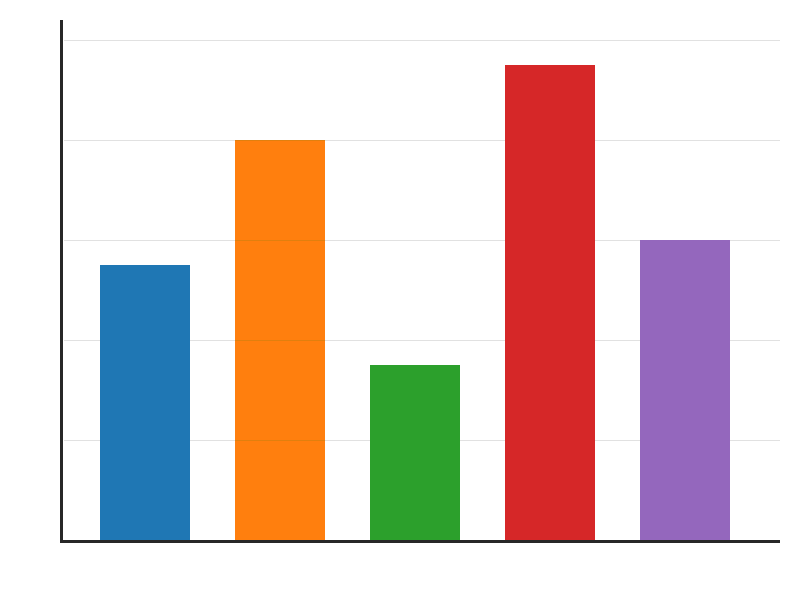
\includegraphics[width=0.35\textwidth]{plot.png}

  A chart of five groups.
\end{frame}

\end{document}
